\begin{itemize}
    \item Create a learning plan based on what you want to do.
    \item Learn the fundamentals and necessary technologies.
    \item Watch tutorials/courses/etc but be sure to create your own personal projects based on what you learn.
    \item Create a portfolio.
    \item Start applying for jobs or finding clients.
\end{itemize}

\section{Learning Plan}

\begin{figure}[H]
    \centering
    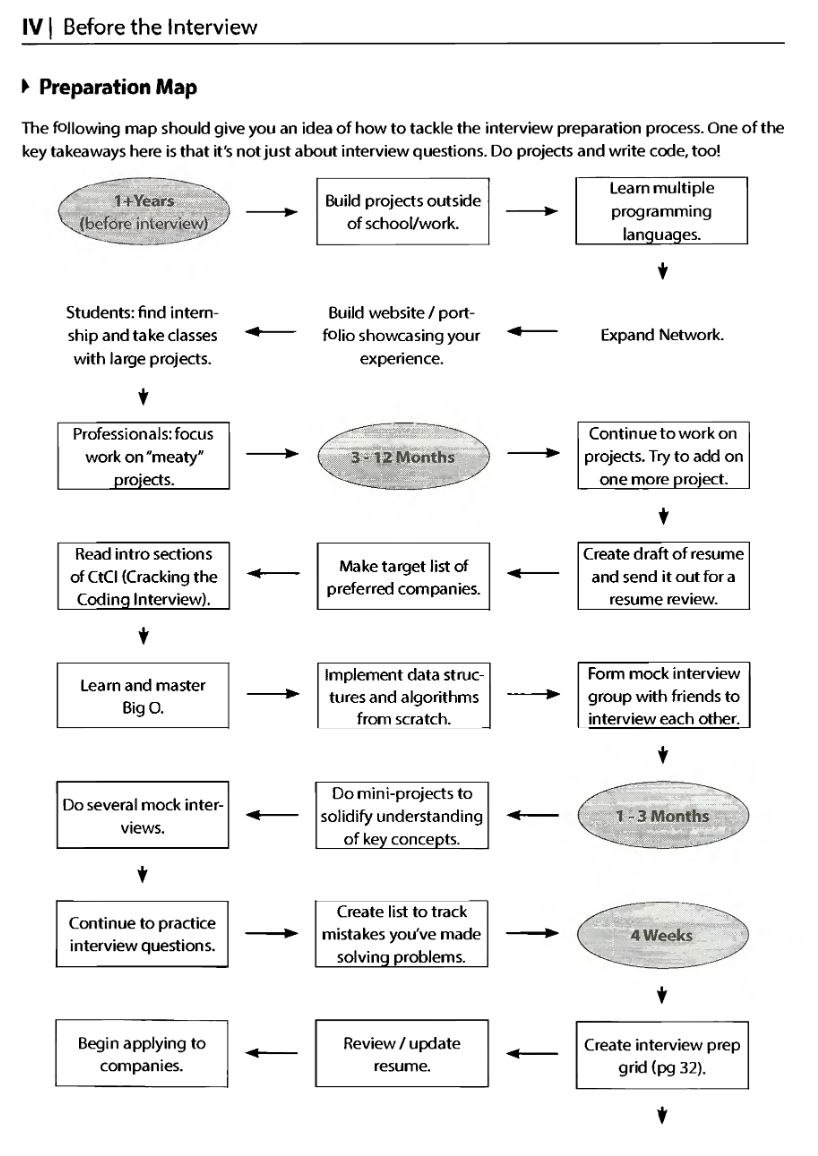
\includegraphics[width=\textwidth]{images/Roadmap 1.png}
    \caption{Roadmap Part 1}
    \label{fig:my_label}
\end{figure}
\begin{figure}[H]
    \centering
    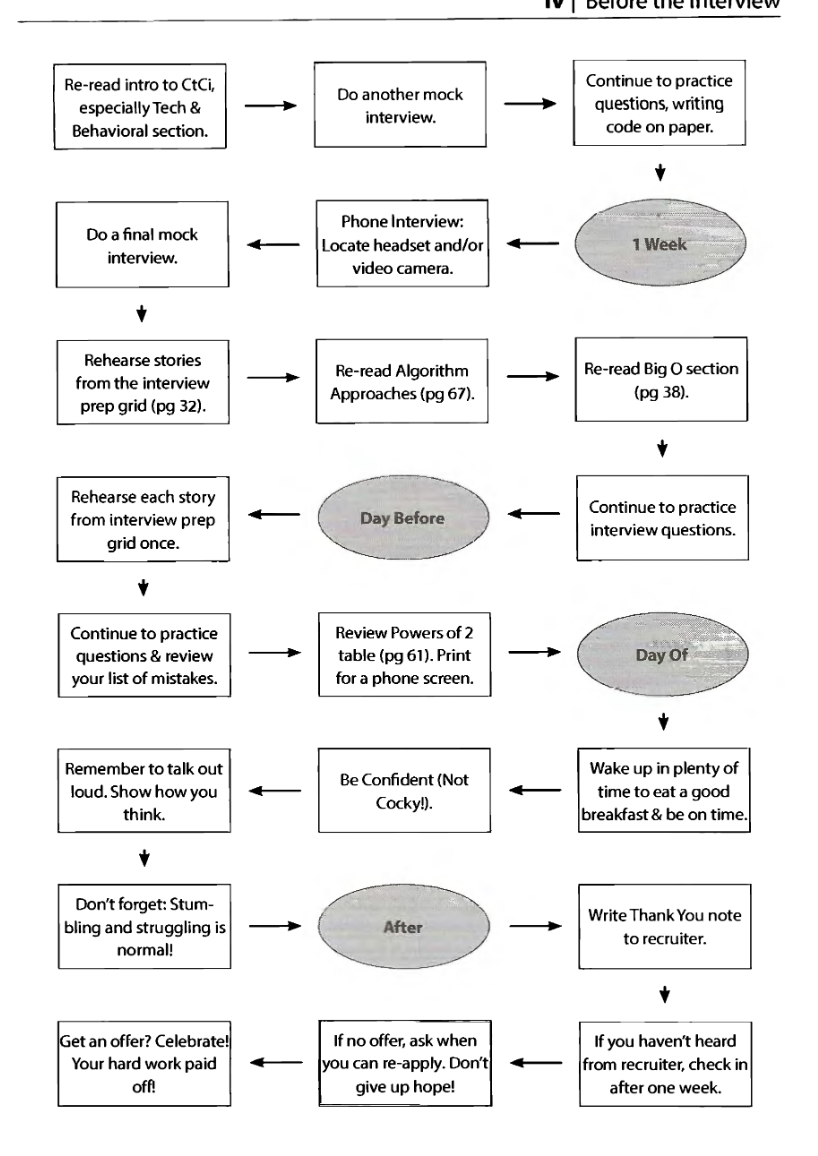
\includegraphics[width=\textwidth]{images/Roadmap 2 .png}
    \caption{Roadmap Part 2}
    \label{fig:my_label}
\end{figure}
\begin{enumerate}
    \item Learn the building blocks.
    \begin{itemize}
        \item Code academy courses: Responsive Web Design, JS Algorithms and Data Structures, front-end development libraries.
    \end{itemize}
    \item Be a front-end superstar.
    \item Follow \emph{Crack the Coding Interview} roadmap.
\end{enumerate}

\section{Example Job Postings}
\subsection*{Front-End}

\subsubsection{Qualifications and Skills}
\begin{itemize}
    \item Collaborate with back end, product and design teams
    \item Own responsibility for overall front end architecture
    \item Communicating tradeoffs with stakeholders, executives, sales/marketing.
    \item While 100\% remote role, availability for meetings U.S. Pacific Time.
\end{itemize}

\subsubsection{Responsibilities}
\begin{itemize}
    \item Minimum of 4 years of software architecture and development experience with at least 1-2 years of lead or principal responsibilities in a data-centric enterprise platform.
    \item Expert experience with Javascript, GraphQL, React, and React Hooks
    \item Substantial startup experience and/or a track record of success in a fast-paced environment.
    \item You make smart architectural decisions, build efficient systems, and have know-how to test and monitor the platforms.
    \item A track record of taking measured risks and providing robust backup and rollback plans.
    \item A track record of moving fast, while proactively managing technical debt and continuous refactoring.
\end{itemize}


\subsection*{Back-End}
\subsubsection{Qualifications and Skills}
\begin{itemize}
    \item Minimum of 5 years of software architecture and development experience with at least 1-2 years of lead or principal responsibilities in a data-centric enterprise platform.
    \item Expert experience with Python OR Go
    \item Significant experience in search, API data services, and performance optimization
    \item Substantial startup experience and/or a track record of success in a fast-paced environment.
    \item You make smart architectural decisions, build efficient systems, and have know-how to test and monitor the platforms.
    \item A track record of taking measured risks and providing robust backup and rollback plans.
    \item A track record of moving fast, while proactively managing technical debt and continuous refactoring.
    \item Bonus for experience with GCP, BigQuery, Redis, jhub/Jupyter Notebook, web scraping tools and Kubernetes
\end{itemize}
\subsubsection{Responsibilities}
\begin{itemize}
    \item Responsible for overall architecture including API design
    \item Search algorithms and performance, e.g. elastic search, entity \& document search.
    \item Data schemas and persistence, data importers.
    \item Machine learning processing pipeline.
    \item Operations: Kubernetes, Monitoring \& Alerting, GCP Resources
    \item Dev tools: Github actions, Makefiles, Release process/scripts
    \item Communicating tradeoffs with stakeholders, executives, sales/marketing.
    \item While 100\% remote role, availability for meetings U.S. Pacific Time.
\end{itemize}
\subsection*{Full Stack}
\subsubsection*{Essential Duties and Responsibilities}

\begin{itemize}
    \item Lead and participate in requirements gathering discussions and document application specifications.
    \item Architect, develop, test, deploy, maintain full-stack customer-facing cloud-based applications (front-end and back-end).
    \item Develop and manage well-functioning databases and applications.
    \item Deliver superior performance for customers ensuring all applications are responsive and fast.
    \item Ensure and manage multiple integrations between O\&O applications and 3rd party SaaS and application platforms.
    \item Write clear, and thorough technical documentation for all developed applications.
    \item Test, troubleshoot, debug and upgrade application software and code as needed.
    \item Manage individual project priorities, deadlines, and deliverables in a flexible work environment.
    \item Participate with other technologists and developers to develop forward-thinking strategy, plans, and software throughout Company.
    \item Work closely with the marketing and research and development to ensure application user-experience meets customer needs.
\end{itemize}

\subsubsection*{Education and Experience}
\begin{itemize}
    \item Bachelor’s Degree in Computer Science, or equivalent work experience
    \item At least 5 years of programming experience through work or personal projects with a strong working knowledge of:
        \begin{itemize}
        \item AWS Lambdas, Dynamo, Beanstalk, ElastiCache, ElasticSearch, CloudFront etc.
        \item Relational/Non-Relational DB experience
        \item Node.js
        \item React.js
        \item Python
        \item Django
        \item Flask
        \item JavaScript
        \item User-authentication
        \end{itemize}
\end{itemize}
